\documentclass{sprawozdanie-agh}

\usepackage{float}
\usepackage[utf8]{inputenc}
\usepackage{matlab-prettifier}
\usepackage{siunitx}
\usepackage{booktabs,caption,ragged2e}
\usepackage{physics}

\makeatletter
% ========= Początek Dokumentu ========= 
\begin{document}
% ========= Strona tytułowa ========= 
\przedmiot{Teoria Sterowania II: Ćwiczenia Laboratoryjne}
\tytul{Wytyczne dla Ćwiczenia 7}
\podtytul{Układy Dyskretne}
\kierunek{Automatyke i~Robotyka}
\autor{Dariusz Cieślar, Maciej Różewicz}
\data{Kraków, \today}

\stronatytulowa{}

% ========= Treść Właściwa =========
\section{Cel ćwiczenia}


Celem ćwiczenia jest zapoznanie się z podstawami projektowania systemów sterowania dyskretnych w~czasie.

Systemy dyskretne modeluje się zwykle za pomocą równań \textbf{różnicowych}, co oznacza, że w równaniach występują wyrażenia przesunięte w czasie o wielokrotność pewnego stałego kroku. Ten krok interpretujemy w praktyce jako okres próbkowania w układzie sterowania. 

Do opisu układów dynamicznych stosujemy równania różnicowe \textbf{rekurencyjne}: wartość sygnału w danym momencie zależy od wartości w poprzednich dyskretnych momentach czasu.
Liniowe układy dyskretne można też opisać za pomocą transmitancji opartej na transformacie $\mathcal{Z}$.

Z modelami takimi można spotkać się w~praktyce bardzo często:
\begin{itemize}
    \item każdorazowo przy projektowaniu sterowania cyfrowego
    \item podczas numerycznego rozwiązywania równań różniczkowych (np. symulacja)
    \item gdy model układu został opracowany na podstawie metod identyfikacji i estymacji parametrów w oparciu o pomiary sygnałów w dyskretnych momentach czasu 
\end{itemize} 

W trakcie ćwiczenia zapoznamy się z:
\begin{enumerate}
    \item zależnością między położeniem wartości własnych macierzy stanu a stabilnością układu dyskretnego
    \item doborem okresu próbkowania dla układów sterowania
    \item projektowaniem regulatorów dyskretnych 
\end{enumerate}

\textbf{Uwaga:} w czasie tego ćwiczenia nie będziemy zajmować się wprost numerycznym rozwiązywaniem równań różniczkowych (choć będziemy je wykorzystywać do symulacji).
Niemniej prosimy pamiętać, że schematy różnicowe są podstawowym zakresem programu Teorii Sterowania i były omawiane podczas ćwiczeń audytoryjnych.


%%%%%%%%%%%%%%%%%%%%%%%%%%%%%%%%%%%%%%%%%%%%%%%%%%%%%%%%%%%
\section{Przebieg ćwiczenia}

\subsection{Wartości własne układów dyskretnych}
Proszę przeanalizować zależność między wartością parametru $\lambda \in \mathcal{R}$ a charakterem rozwiązania układu dyskretnego opisanego równaniem:
\begin{equation*}
x(k+1) = \lambda x(k) \qquad k = 0, 1, 2, \ldots
\end{equation*} 
\begin{description}

\item[Krok 1] Dobierz po jednej wartości parametru $\lambda$ dla każdego z następujących przedziałów:
\begin{itemize}
    \item $\lambda < -1$
    \item $\lambda = -1$
    \item $\lambda \in (-1,0)$
    \item $\lambda = 0$
    \item $\lambda \in (0,1)$
    \item $\lambda = 1$
    \item $\lambda > 1$
\end{itemize}
\item[Krok 2] Wykreśl na płaszczyźnie zespolonej koło jednostkowe oraz zaznacz punkty odpowiadające wartościom $\lambda$ wybranym w poprzednim kroku
\item[Krok 3] Dla każdej z wybranych wartości $\lambda$ wykreśl odpowiedź układu na ten sam niezerowy warunek początkowy,
\item[Krok 4] Opisz obserwacje zwracając uwagę na zależność charakteru odpowiedzi od położenia punktu $\lambda$ na płaszczyźnie zespolonej
\end{description}

\subsection{Okres próbkowania i cyfrowy odpowiednik układu ciągłego}
Model matematyczny silnika prądu stałego o schemacie jak na rysunku poniżej
    \begin{figure}[H]
        \centering
        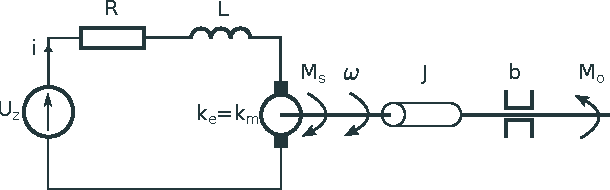
\includegraphics[width=0.5\linewidth]{fig/SilnikDC.pdf}
        \caption{Schemat silnika prądu stałego.}
    \end{figure}
można opisać równaniami:
        \begin{itemize}
            \item Siła elektromotoryczna indukcji: $e = k_e\omega$
            \item Napięciowe prawo Kirchoffa: $iR+\dv{i}{t}L+k_e\omega = U_z$
            \item Moment obrotowy wirnika: $M_s = k_mi$
            \item Równanie momentów dla wirnika: $M_s = k_mi=J\dv{\omega}{dt} + b\omega + M_o$
        \end{itemize}
Model ten można zapisać w~postaci równań stanu:

\begin{align*}
\begin{bmatrix} \dv{i}{t} \\  \dv{\omega}{t} \end{bmatrix} &= \begin{bmatrix} -\frac{R}{L} & -\frac{k_e}{L} \\ \frac{k_m}{J} & -\frac{b}{J} \end{bmatrix}\begin{bmatrix} i \\  \omega \end{bmatrix} + \begin{bmatrix} \frac{1}{L} & 0 \\ 0 & -\frac{1}{J} \end{bmatrix}\begin{bmatrix} U_z \\ M_{o} \end{bmatrix} \\
y &= \begin{bmatrix} 0 & 1  \end{bmatrix} \begin{bmatrix} i \\  \omega \end{bmatrix} + \begin{bmatrix} 0 & 0  \end{bmatrix} \begin{bmatrix} U_z \\ M_{o} \end{bmatrix}
\end{align*}


Skorzystaj ze skryptu \textit{SilnikDC{\_}Dyskretyzacja.mlx} oraz modelu Simulink \textit{SilnikDC{\_}Dyskretyzacja.slx}, aby wykonać następujące kroki:

\begin{description}
\item[Krok 5] Wyznacz pulsację graniczną $\omega_c$ dla układu ciągłego, przy której amplituda charakterystyki częstotliwościowej spada o~3dB
\item[Krok 6] Przeprowadż symulacje dla różnych pulsacji, by zaobserwować efekt utraty amplitudy dla pulsacji wyższych od pasma przenoszenia.
\item[Krok 7] Wyznacz okres próbkowania $h$ adekwatny do projektowania regulatora dyskretnego.
\item[Krok 8] Przeprowadź symulacje dla różnych okresów próbkowania, aby zaobserwować efekt zniekształcania odpowiedzi układu ciągłego przez ZOH. 
\begin{itemize}
    \item zaobserwuj zniekształcenie dla maksymalnego okresu próbkowania wynikającego z~reguły Nyquista-Shannona
    \item spróbuj zaobserwować zjawisko aliasingu
\end{itemize}
\item[Krok 9] Wyznacz dyskretny odpowiednik układu ciągłego przy okresie próbkowania z Kroku 7 i sprawdź czy jego wyjście jest zgodne z wyjściem układu ciągłego.
\end{description}

\subsection{Projektowanie regulatorów dyskretnych}

W tej częsci ćwiczenia zajmiemy się projektowaniem regulatorów dyskretnych. Można to zrobić na dwa sposoby pokazane na poniższym rysunku.
    \begin{figure}[H]
        \centering
        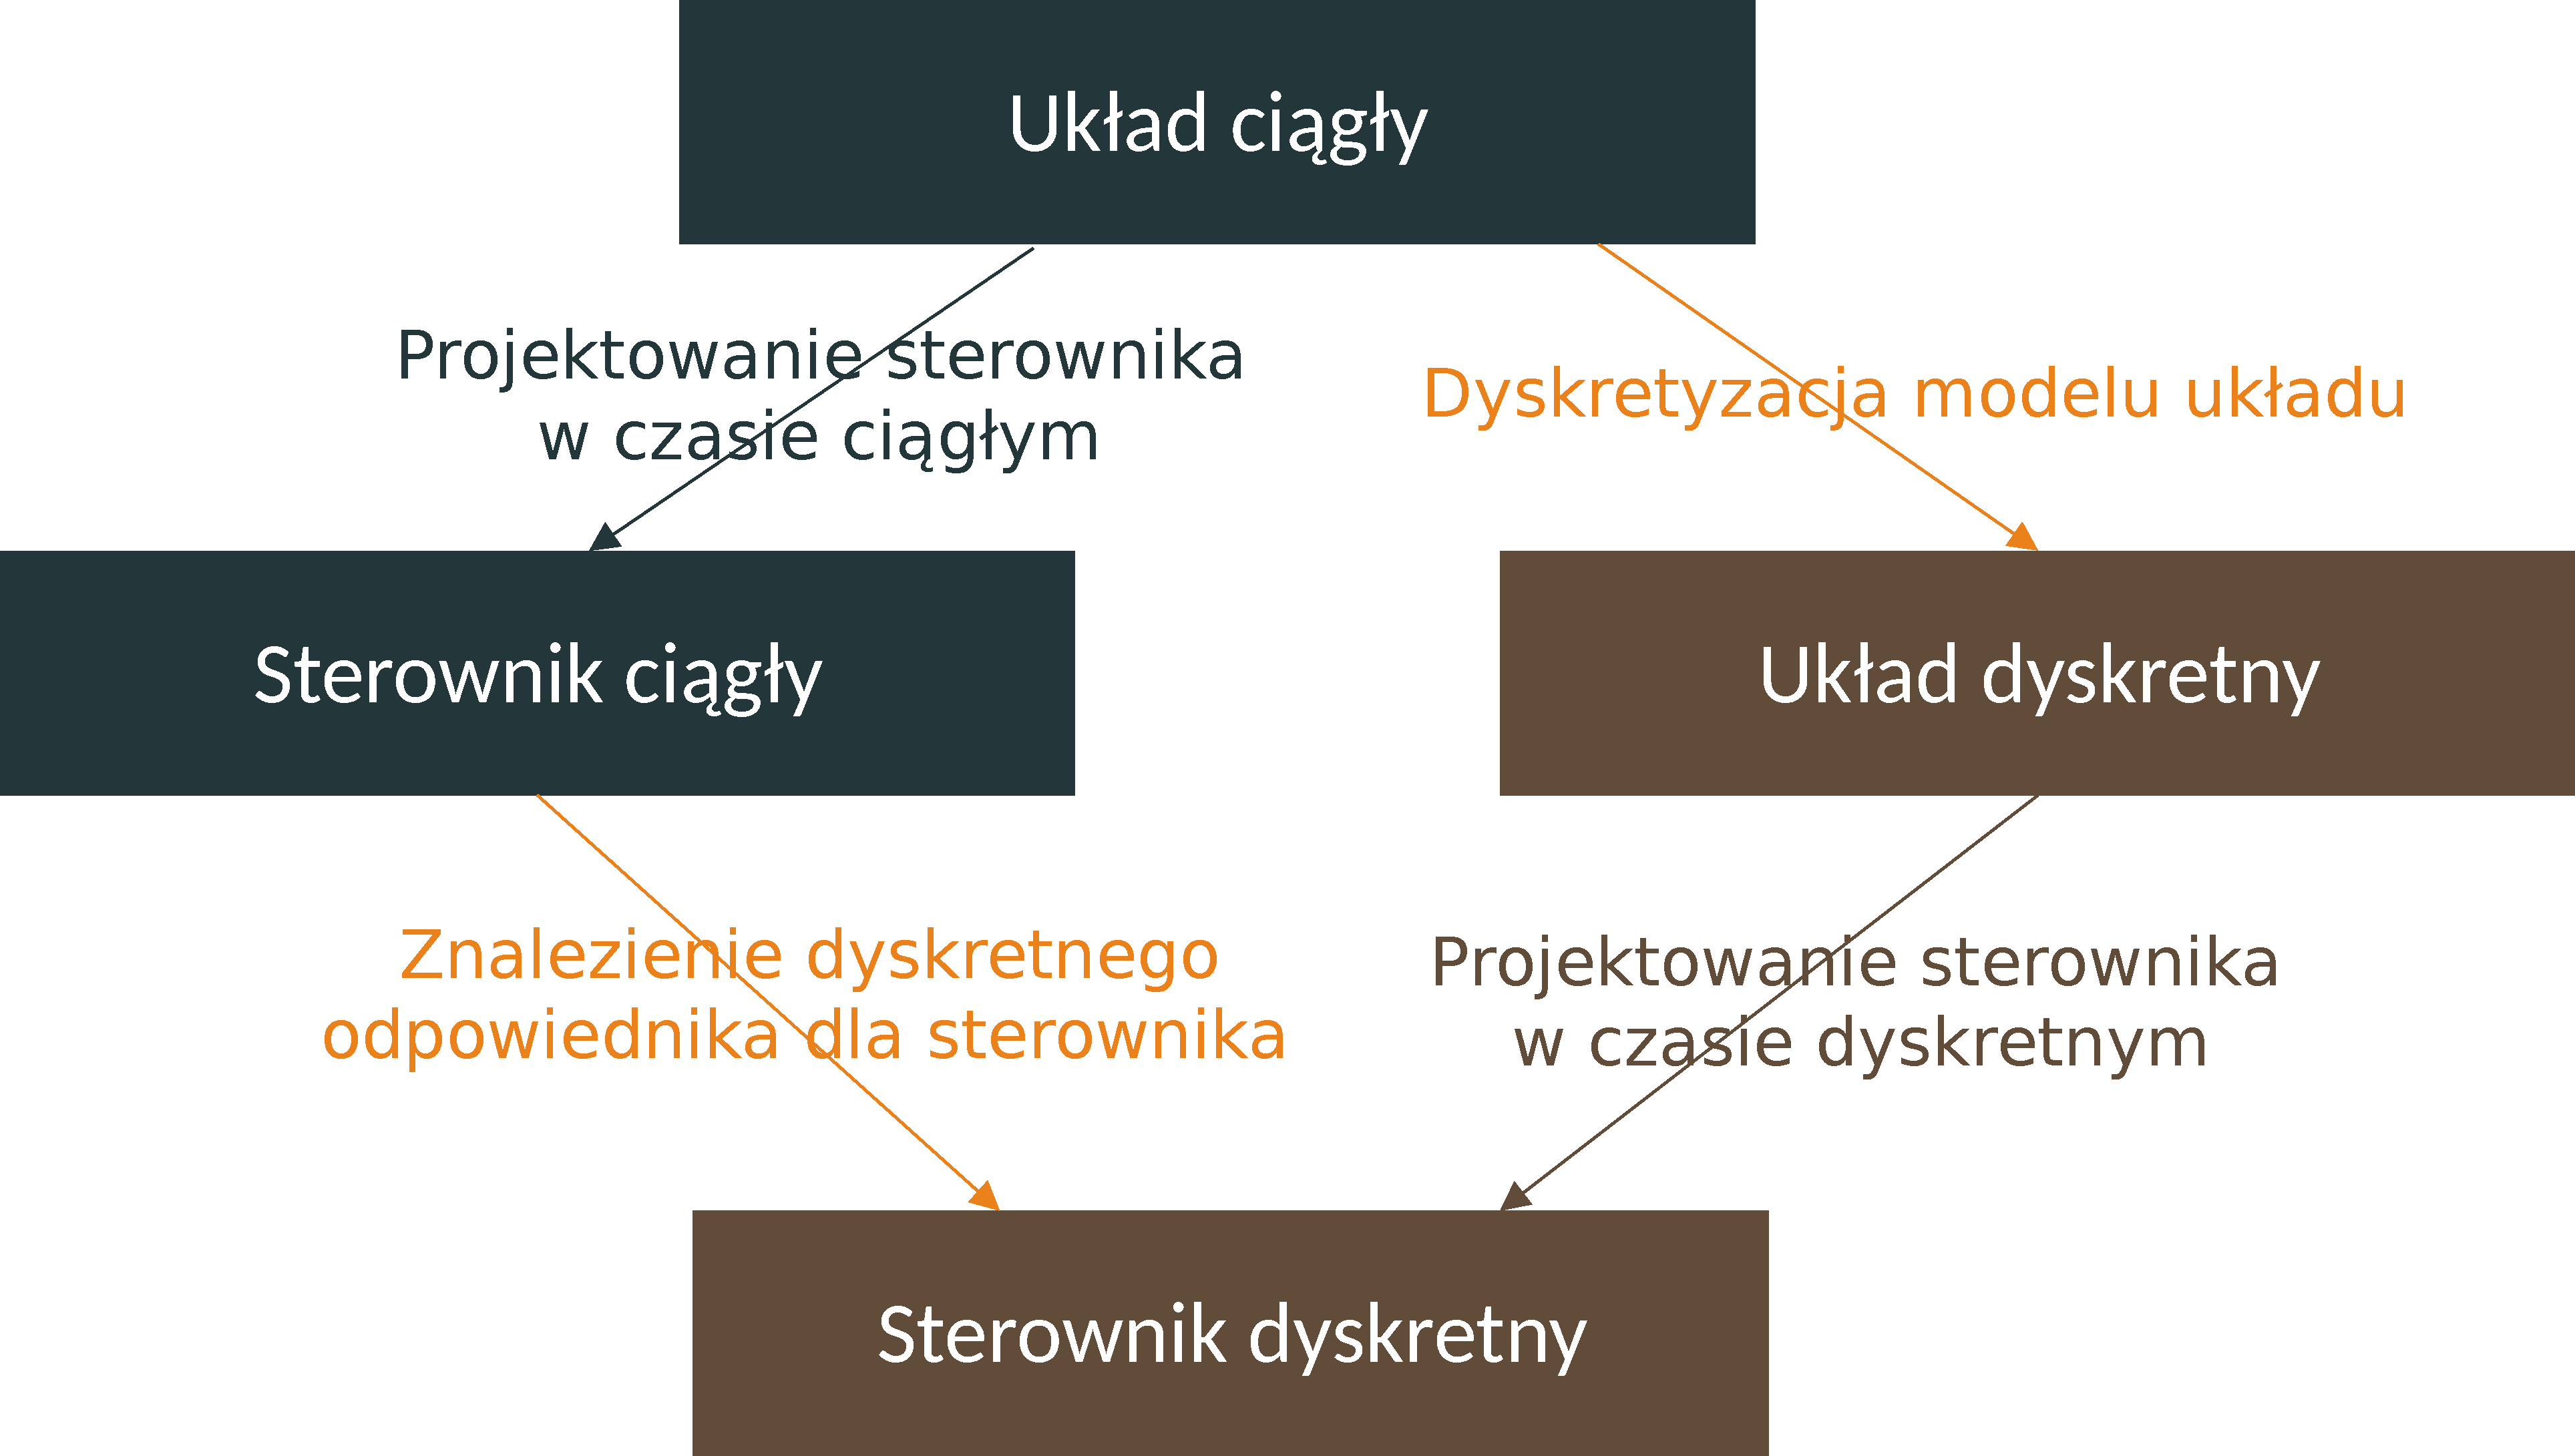
\includegraphics[width=0.5\linewidth]{fig/Cont2Disc.pdf}
        \caption{Dwie ścieżki projektowania układów ze sterownikiem dyskretnym.}
        
    \end{figure}

W trakcie tego ćwiczenia zajmiemy się ścieżką po lewej stronie rysunku, czyli zaprojektujemy regulator w czasie ciągłym, a następnie znajdziemy jego odpowiednik dyskretny.

Na początku rozszerzymy model silnika prądu stałego o sygnał kąta obrotu wału $\theta$. Będzie on traktowany jako pomiar służący do sterowania, a~napięcie $U_z$ potraktujemy jako wejście sterujące. Otrzymujemy w~ten sposób układ o~postaci:
\begin{align*}
\begin{bmatrix} \dv{i}{t} \\  \dv{\omega}{t} \\ \dv{\theta}{t} \end{bmatrix} &= \begin{bmatrix} -\frac{R}{L} & -\frac{k_e}{L} & 0\\ \frac{k_m}{J} & -\frac{b}{J} & 0 \\ 0 & 1 & 0\end{bmatrix}\begin{bmatrix} i \\  \omega \\ \theta \end{bmatrix} + \begin{bmatrix} \frac{1}{L} \\ 0 \end{bmatrix} U_z  \\
y &= \begin{bmatrix} 0 & 0 &1  \end{bmatrix} \begin{bmatrix} i \\  \omega \\ \theta \end{bmatrix} + \begin{bmatrix} 0  \end{bmatrix} U_z 
\end{align*}

Układ będziemy sterować za pomocą regulatora PD w celu uzyskania funkcjonalności serwomechanizmu, czyli śledzenia zadanej trajektorii kąta obrotu $\theta$.
W czasie ciągłym regulator PD ustalimy w postaci:
\begin{equation*}
u(t) = k_p \left(e(t) + 0.1 \dv{e(t)}{t}\right)
\end{equation*}
Transmitancja tego regulatora PD to:
\begin{equation*}
K(s) = k_p \left(1 + 0.1s\right)
\end{equation*}
Skorzystaj ze skryptu \textit{Serwo{\_}RegulatorDyskretny.mlx} oraz modelu Simulink \textit{Serwo{\_}RegulatorDyskretny.slx}, aby wykonać następujące kroki:
Eksperymenty rozpocznij z okresem próbkowania $h$ wyznaczonym w poprzedniej części ćwiczenia.

\begin{description}
\item[Krok 10] Wyznacz zakres wzmocnienia $k_p$, dla którego układ serwo jest stabilny w czasie ciągłym.
\item[Krok 11] Wyznacz sterownik dyskretny wykorzystując aproksymację Tustina, a~następnie wyznacz zakres wzmocnienia $k_p$, dla którego układ serwo jest stabilny w czasie dyskretnym.
\item[Krok 12] Przeprowadź symulacje dla wybranej wartości $k_p$ zapewniającej stabilność regulatorów w czasie ciągłym i dyskretnym, aby zbadać wpływ dyskretyzacji na zachowanie układu.
\item[Krok 13] Przeprowadź symulacje dla maksymalnych wartości $k_p$ (innych dla regulatora ciągłego i dyskretnego) zapewniających stabilność i sprawdź zachowanie układów.
\item[Krok 14] Sprawdź jak zmienia się zakres stabilności wzmocnienia $k_p$ dla różnych okresów próbkowania (zmieniając domyślną wartość $h$). Swoje obserwacje zilustruj wykresami przebiegów czasowych i pozycji wartości własnych układu dyskretnego.
\end{description}

\section{Opracowanie wyników}

Przygotuj sprawozdanie z ćwiczenia opisujące cel, przebieg i obserwacje.


W części opisującej przebieg koniecznie należy zawrzeć:
\begin{itemize}
    \item wykresy pozycji wybranych $\lambda$ na płaszczyźnie zespolonej z Kroku 2
    \item wykresy odpowiedzi dla wybranych $\lambda$, czyli ilustracje z Kroku 3
    \item wykres ilustrujący efekt utraty amplitudy dla pulsacji wyższych od pasma przenoszenia z Kroku 6
    \item wykresy ilustrujące efekt zniekształcania odpowiedzi układu ciągłego dla maksymalnego okresu próbkowania wynikającego z~reguły Nyquista-Shannona z Kroku 8
    \item wykresy porównujące odpowiedzi układu ciągłego i dyskretnego z Kroku 9
    \item wartości $k_p$ zapewniające stabilność regulatorów w czasie ciągłym i dyskretnym z Kroku 10 i Kroku 11
    \item wykresy porównujące odpowiedzi układu dla wybranego $k_p$ zastosowanego do sterownika ciągłego i dyskretnego z Kroku 12
    \item wykresy ilustrujące wpływ okresu próbkowania $h$ na układ zamknięty, czyli wykresy przebiegów czasowych i pozycji wartości własnych układu dyskretnego z Kroku 14
\end{itemize}

\end{document}


